\section{解析手順}
\href{https://ofbkansai.sakura.ne.jp/}{オープンCAE勉強会@関西公式HP}のARCHIVE「これまでの勉強会と発表資料」にあるmmer547氏の第59回での発表資料「Salome-Mecaで熱応力解析(Salome-Meca復習シリーズ)」では、一つのコマンドファイルで熱解析と熱応力解析を実施していたのに対し、今回は熱解析の結果を構造解析で読み込み、熱応力解析を実施してみました。
\vspace{-0.5\baselineskip}
\begin{table}[H]
	\centering
	\begin{tabular}{p{30mm}p{60mm}p{45mm}p{50mm}p{40mm}}
		\toprule
		ステップ &                      &                          & 使用モジュール & 備考               \\ \midrule
		共通     & 1.ジオメトリ定義     &                          & Geom/Shaper    &                    \\ \cline{2-5}
		         & 2.メッシュ生成       &                          & Mesh           &                    \\ \midrule
		熱解析   & 3.データ設定         & コマンドファイル雛形作成 & AsterStudy     & Assistant使用      \\ \cline{2-5}
		         & 4.求解               &                          & AsterStudy     &                    \\ \cline{2-5}
		         & 5.結果分析(可視化) &                          & ParaVis        &                    \\ \midrule
		構造解析 & 6.データ設定         & コマンドファイル雛形作成 & AsterStudy     & Assistant使用      \\ \cline{3-5}
		         &                      & コマンドファイル編集     & AsterStudy     & 熱解析の結果を継承 \\ \cline{2-5}
		         & 7.求解               &                          & AsterStudy     &                    \\ \cline{2-5}
		         & 8.結果分析(可視化) &                          & ParaVis        &                    \\ \midrule
	\end{tabular}
\end{table}
\section{Salome-Mecaでモデル作成}
\vspace{-\baselineskip}
\begin{figure}[H]
	\begin{minipage}{0.49\hsize}
		\begin{itemize}
			\item ジオメトリ
			      \begin{itemize}
				      \item 直方体:X=100mm、Y=Z=10mm
			      \end{itemize}
			\item メッシュ
			      \begin{itemize}
				      \item 六面体一次要素
				      \item メッシュサイズ:10mm
			      \end{itemize}
		\end{itemize}
	\end{minipage}
	\begin{minipage}{0.49\hsize}
		\begin{itemize}
			\item グループ化
			      \begin{itemize}
				      \item Groups of Faces(Elements)
				            \begin{itemize}
					            \item Fix\_X1、Fix\_X2
				            \end{itemize}
				      \item Groups of Nodes
				            \begin{itemize}
					            \item Fix\_Y、Fix\_Z
				            \end{itemize}
			      \end{itemize}
		\end{itemize}
	\end{minipage}
\end{figure}
\vspace{-\baselineskip}
\begin{figure}[H]
	% 	\caption{}
	% 	\label{}
	\centering
	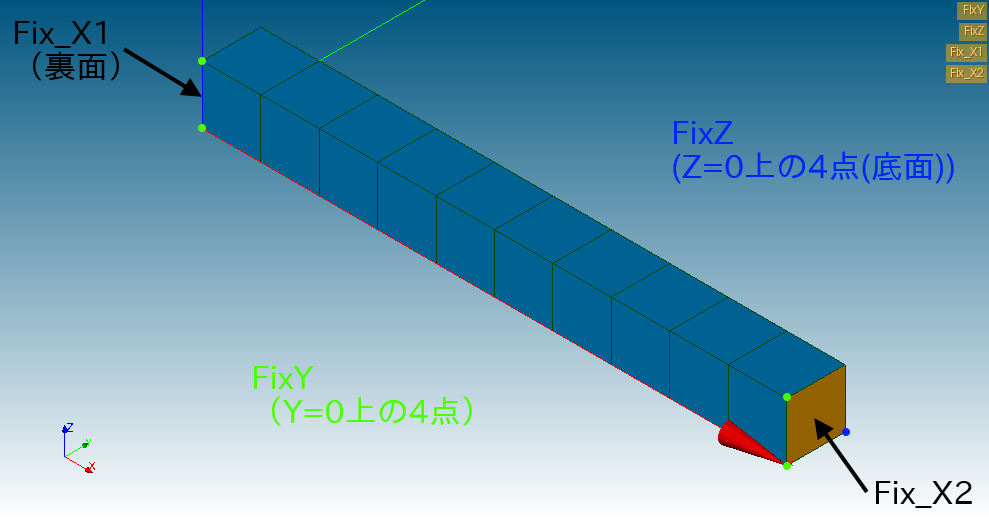
\includegraphics[width=0.9\columnwidth]{fig/model.png}
\end{figure}
\section{Salome-Mecaで熱解析を実施}
\subsection{熱解析の設定}
\begin{figure}[H]
	\begin{minipage}{0.49\hsize}
		\begin{itemize}
			\item 検証問題
			      \begin{itemize}
				      \item 両端の面を100℃に固定
				      \item それ以外の面は断熱条件(熱条件なし)
				      \item 定常熱伝導
			      \end{itemize}
		\end{itemize}
	\end{minipage}
	\begin{minipage}{0.49\hsize}
		\begin{itemize}
			\item 材料定数
			      \begin{itemize}
				      \item 熱伝導率$\lambda$:0.016 [W/(mm・K)]
				            \vspace{2\baselineskip}
			      \end{itemize}
		\end{itemize}
	\end{minipage}
\end{figure}
\begin{figure}[H]
	% 	\caption{}
	% 	\label{}
	\centering
	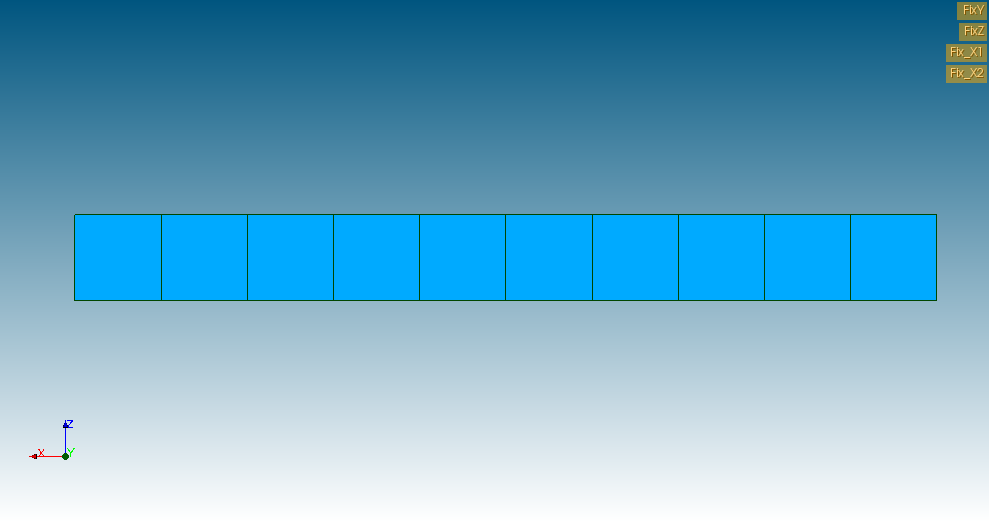
\includegraphics[width=0.6\columnwidth]{fig/setting.png}
\end{figure}
\subsection{AsterStudyで熱解析の設定(Assisantを使用)}
\begin{itemize}
	\item AsterStudyモジュールを起動
	\item メニューより、\menu[,]{Operations,Add Stage with Assitant,Liner Thermal Analysis}を選択
	\item イントロダクションが表示されるので、\keys{Next>}をクリック
	      \begin{figure}[H]
		      % 	\caption{}
		      % 	\label{}
		      \centering
		      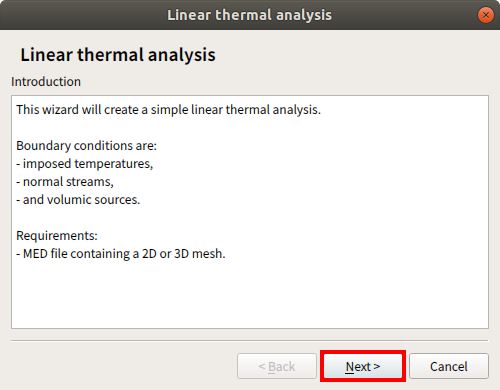
\includegraphics{fig/Assisant_thermal_001.png}
	      \end{figure}
	      \clearpage
	\item 作成したメッシュを選択し、\keys{Next>}をクリック
	      \begin{figure}[H]
		      % 	\caption{}
		      % 	\label{}
		      \centering
		      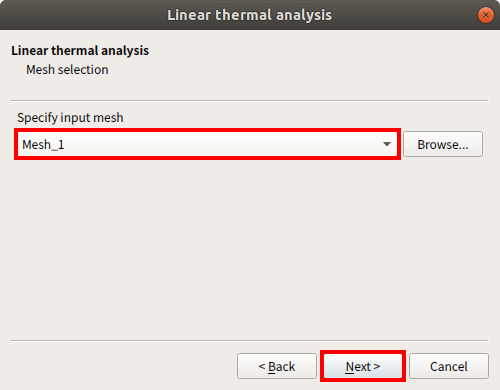
\includegraphics{fig/Assisant_thermal_002.png}
	      \end{figure}
	      \clearpage
	\item モデルは3Dを選択し、\keys{Next>}をクリック
	      \begin{figure}[H]
		      % 	\caption{}
		      % 	\label{}
		      \centering
		      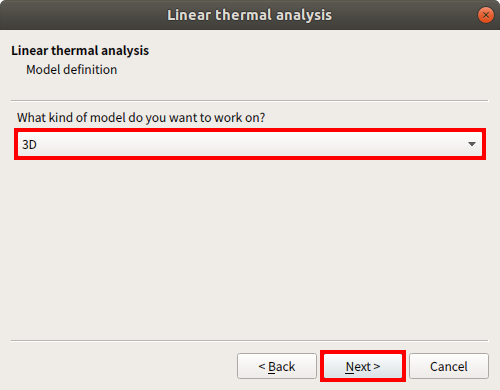
\includegraphics{fig/Assisant_thermal_003.png}
	      \end{figure}
	      \clearpage
	\item 熱伝導率$\lambda$:0.016 [W/(mm・K)]を入力し、\keys{Next>}をクリック
	      \begin{figure}[H]
		      % 	\caption{}
		      % 	\label{}
		      \centering
		      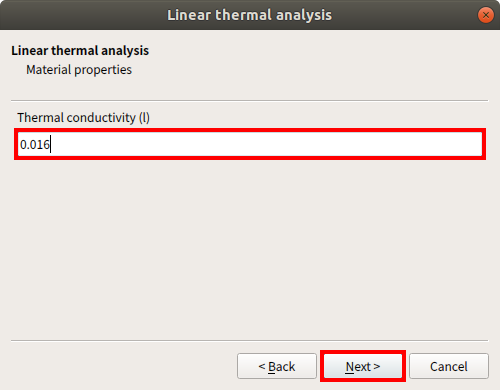
\includegraphics{fig/Assisant_thermal_004.png}
	      \end{figure}
	      \clearpage
	\item 温度条件としてFix\_X1とFix\_X2に100℃を入力し、\keys{Next>}をクリック
	      \begin{figure}[H]
		      % 	\caption{}
		      % 	\label{}
		      \centering
		      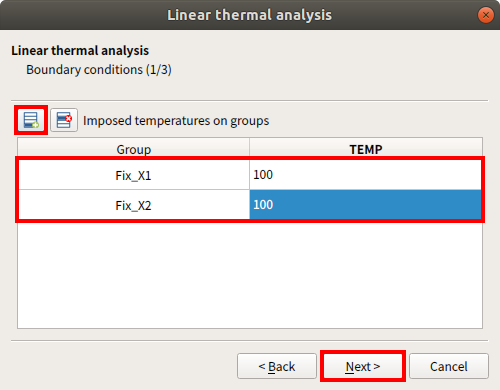
\includegraphics{fig/Assisant_thermal_005.png}
	      \end{figure}
	      \clearpage
	\item 熱流速の定義
	      \begin{itemize}
		      \item 今回は使いませんので、「No」を選択し、\keys{Next>}をクリック
	      \end{itemize}
	      \begin{figure}[H]
		      % 	\caption{}
		      % 	\label{}
		      \centering
		      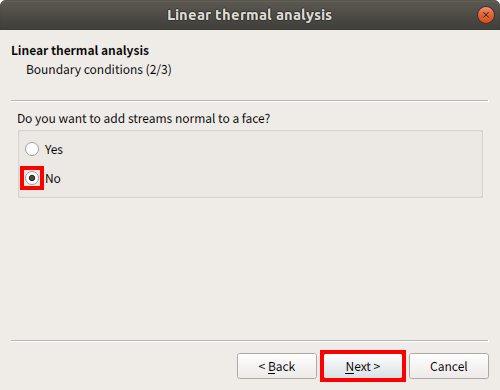
\includegraphics{fig/Assisant_thermal_006.png}
	      \end{figure}
	      \clearpage
	\item 発熱量の定義
	      \begin{itemize}
		      \item 今回は使いませんので、「No」を選択し、\keys{Next>}をクリック
	      \end{itemize}
	      \begin{figure}[H]
		      % 	\caption{}
		      % 	\label{}
		      \centering
		      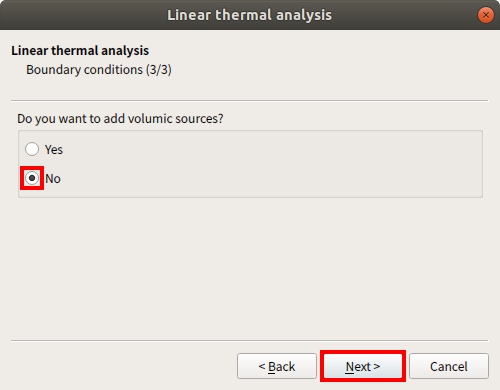
\includegraphics{fig/Assisant_thermal_007.png}
	      \end{figure}
	      \clearpage
	\item 結果ファイル(.rmed)を保存し、\keys{Finish}をクリック
	      \begin{figure}[H]
		      % 	\caption{}
		      % 	\label{}
		      \centering
		      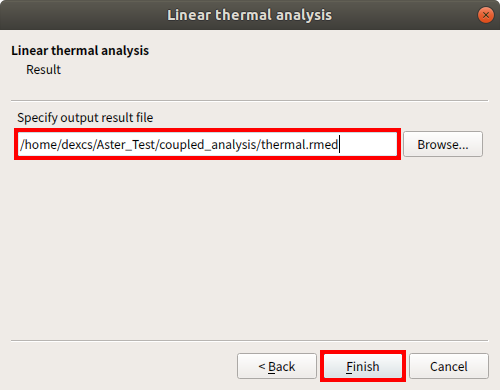
\includegraphics{fig/Assisant_thermal_008.png}
	      \end{figure}
\end{itemize}
\clearpage
\subsection{Assisantで設定した熱解析のコマンドファイル}
次のコマンドファイルがAssisantで設定した熱解析のコマンドファイルです。\\
今回は編集なしで、そのまま解析を実施します。
\begin{lstlisting}[caption =熱解析コマンドファイル, label=コマンドファイル]
DEBUT(LANG='EN')

mesh = LIRE_MAILLAGE(FORMAT='MED',
                     UNITE=20)

model = AFFE_MODELE(AFFE=_F(MODELISATION='3D',
                            PHENOMENE='THERMIQUE',
                            TOUT='OUI'),
                    MAILLAGE=mesh)

mater = DEFI_MATERIAU(THER=_F(LAMBDA=0.016))

matfield = AFFE_MATERIAU(AFFE=_F(MATER=mater,
                                 TOUT='OUI'),
                         MAILLAGE=mesh)

loadst = AFFE_CHAR_THER(MODELE=model,
                        TEMP_IMPO=(_F(GROUP_MA=('Fix_X1', ),
                                      TEMP=100.0),
                                   _F(GROUP_MA=('Fix_X2', ),
                                      TEMP=100.0)))

temp = THER_LINEAIRE(CHAM_MATER=matfield,
                     EXCIT=_F(CHARGE=loadst),
                     MODELE=model)

IMPR_RESU(FORMAT='MED',
          RESU=_F(RESULTAT=temp),
          UNITE=80)

FIN()
\end{lstlisting}
\clearpage
\subsection{Paravisで結果分析(可視化)}
\begin{itemize}
	\item 温度は両端一定なので100℃
\end{itemize}
\vspace{-\baselineskip}
\begin{figure}[H]
	% 	\caption{}
	% 	\label{}
	\centering
	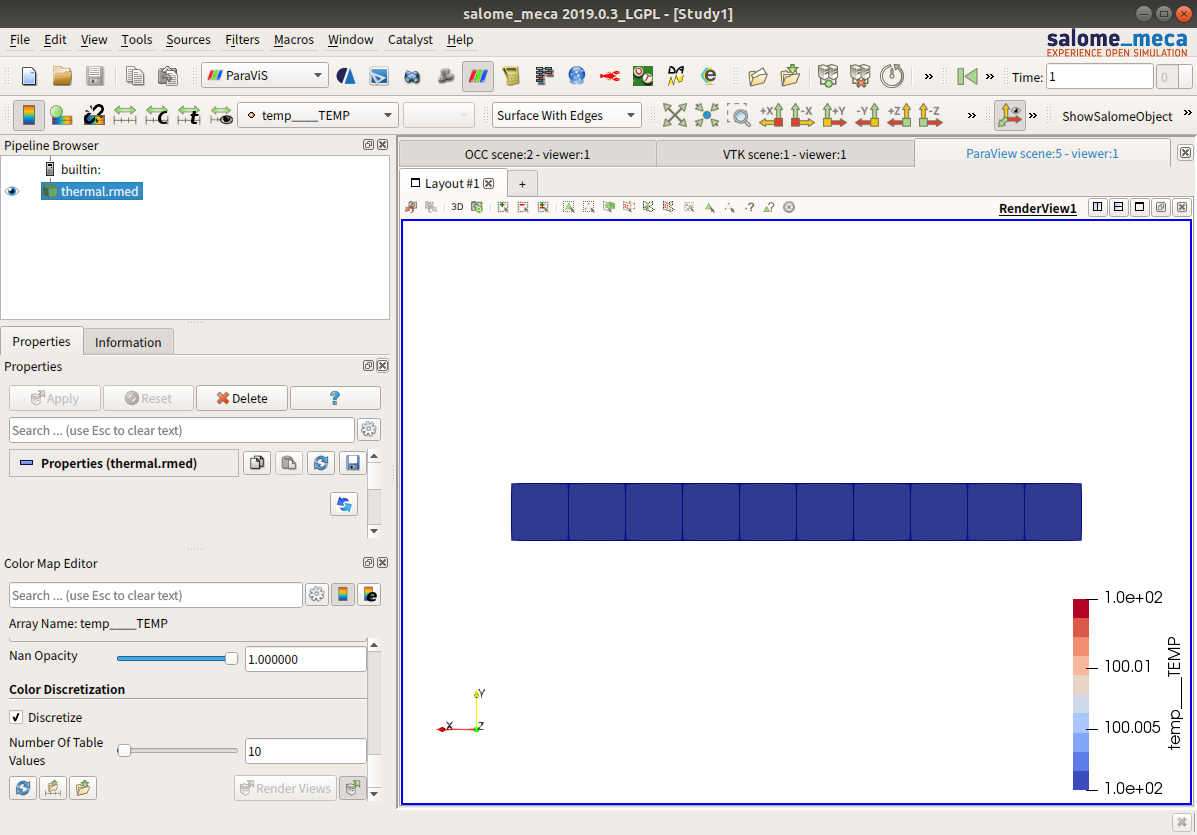
\includegraphics[width=0.8\columnwidth]{fig/thermal.png}
\end{figure}
\clearpage
\section{Salome-Mecaで熱応力解析を実施}
\subsection{構造解析の設定}
\vspace{-\baselineskip}
\begin{figure}[H]
	\begin{minipage}{0.59\hsize}
		\begin{itemize}
			\item 検証問題
			      \begin{itemize}
				      \item 変位拘束
				            \begin{itemize}
					            \item Fix\_X1、Fix\_X2にDX=0
					            \item Fix\_YにDY=0
					            \item Fix\_ZにDZ=0
				            \end{itemize}
				      \item 定常熱伝導問題を解いた結果(温度分布)を継承
				      \item 参照温度を20℃に設定
			      \end{itemize}
		\end{itemize}
	\end{minipage}
	\begin{minipage}{0.39\hsize}
		\begin{itemize}
			\item 材料定数
			      \begin{itemize}
				      \item ヤング率\textit{E}:203,000 [MPa]
				      \item ポアソン比$\nu$:0.3
				      \item 線膨張係数$\alpha$:1.73×$10^{-5}$ [1/℃]
			      \end{itemize}
		\end{itemize}
		\vspace{2\baselineskip}
	\end{minipage}
\end{figure}
\vspace{-\baselineskip}
\begin{figure}[H]
	% 	\caption{}
	% 	\label{}
	\centering
	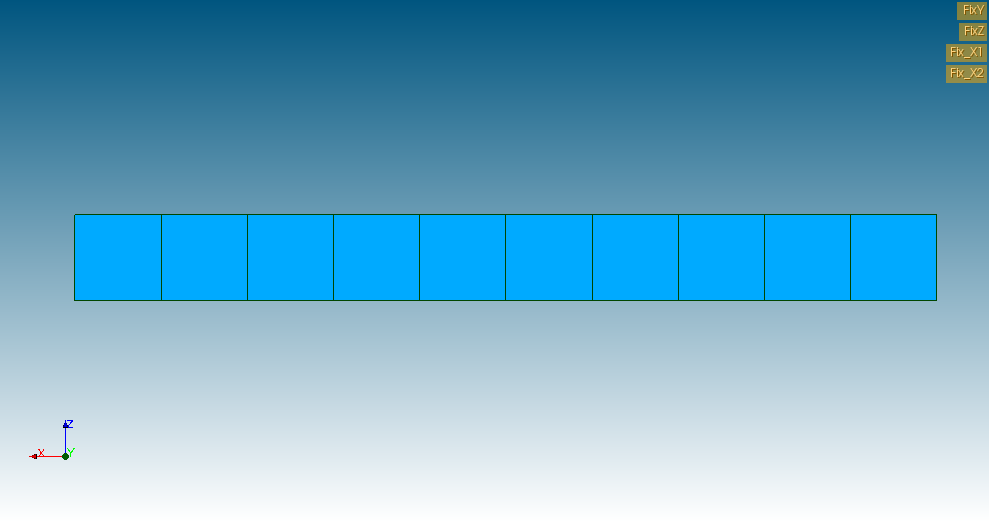
\includegraphics[width=0.6\columnwidth]{fig/settingS.png}
\end{figure}
\clearpage
\subsection{AsterStudyで構造解析の設定(Assisantを使用)}
\begin{itemize}
	\item AsterStudyモジュールの「Case View」タブに戻り、
	\item メニューより、\menu[,]{Operations,Add Stage with Assitant,Isotropic liner elasticity}を選択
	\item イントロダクションが表示されるので、\keys{Next>}をクリック
	      \begin{figure}[H]
		      % 	\caption{}
		      % 	\label{}
		      \centering
		      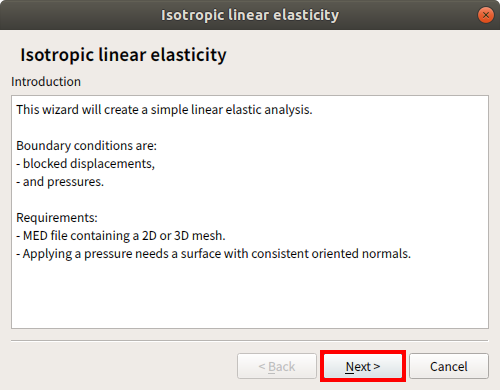
\includegraphics{fig/meca001.png}
	      \end{figure}
	      \clearpage
	\item 作成したメッシュを選択し、\keys{Next>}をクリック
	      \begin{figure}[H]
		      % 	\caption{}
		      % 	\label{}
		      \centering
		      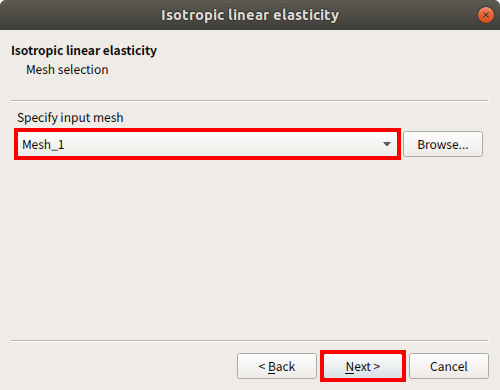
\includegraphics{fig/meca002.png}
	      \end{figure}
	      \clearpage
	\item モデルは3Dを選択し、\keys{Next>}をクリック
	      \begin{figure}[H]
		      % 	\caption{}
		      % 	\label{}
		      \centering
		      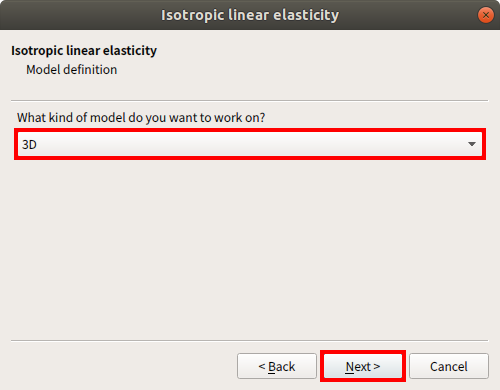
\includegraphics{fig/meca003.png}
	      \end{figure}
	      \clearpage
	\item ヤング率\textit{E}:203,000 [MPa]とポアソン比$\nu$:0.3を入力し、\keys{Next>}をクリック
	      \begin{figure}[H]
		      % 	\caption{}
		      % 	\label{}
		      \centering
		      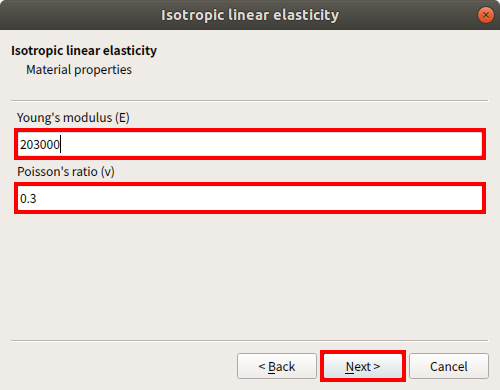
\includegraphics{fig/meca004.png}
	      \end{figure}
	      \clearpage
	\item 拘束条件としてFix\_X1とFix\_X2にDX=0を入力し、\keys{Next>}をクリック
	      \begin{figure}[H]
		      % 	\caption{}
		      % 	\label{}
		      \centering
		      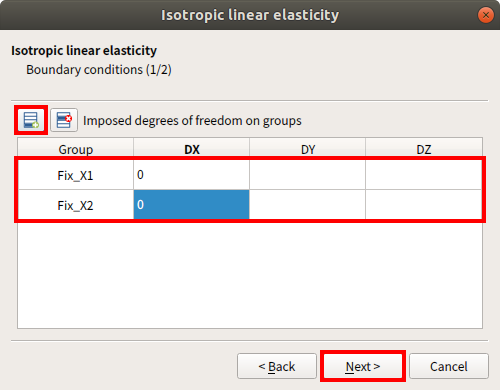
\includegraphics{fig/meca005.png}
	      \end{figure}
	      \clearpage
	\item 荷重条件(圧力条件)
	      \begin{itemize}
		      \item 今回は使いませんので、Assitantでは適当な値を入力(後ほどコマンドファイルを編集して削除します)し、\keys{Next>}をクリック
	      \end{itemize}
	      \begin{figure}[H]
		      % 	\caption{}
		      % 	\label{}
		      \centering
		      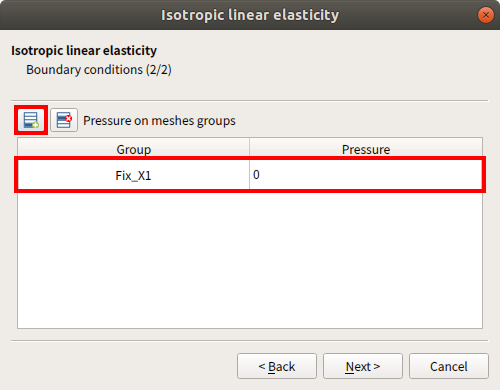
\includegraphics{fig/meca006.png}
	      \end{figure}
	      \clearpage
	\item 結果ファイル(.rmed)を保存し、\keys{Finish}をクリック
	      \begin{figure}[H]
		      % 	\caption{}
		      % 	\label{}
		      \centering
		      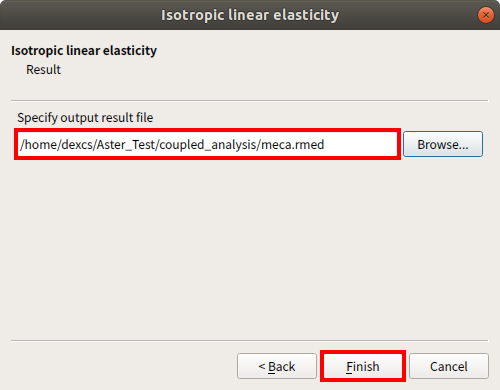
\includegraphics{fig/meca007.png}
	      \end{figure}
\end{itemize}
\clearpage
\subsection{Assisantで設定した構造解析のコマンドファイルを編集}
AssisantのIsotropic liner elasticityで設定したデフォルトのコマンドファイルでは、先に設定したStage\_1熱解析コマンドファイルの設定と、同一の解析ケース内に重複する設定があることになり、Stage\_2のコマンドファイル編集が必要。
\begin{figure}[H]
	% 	\caption{}
	% 	\label{}
	\centering
	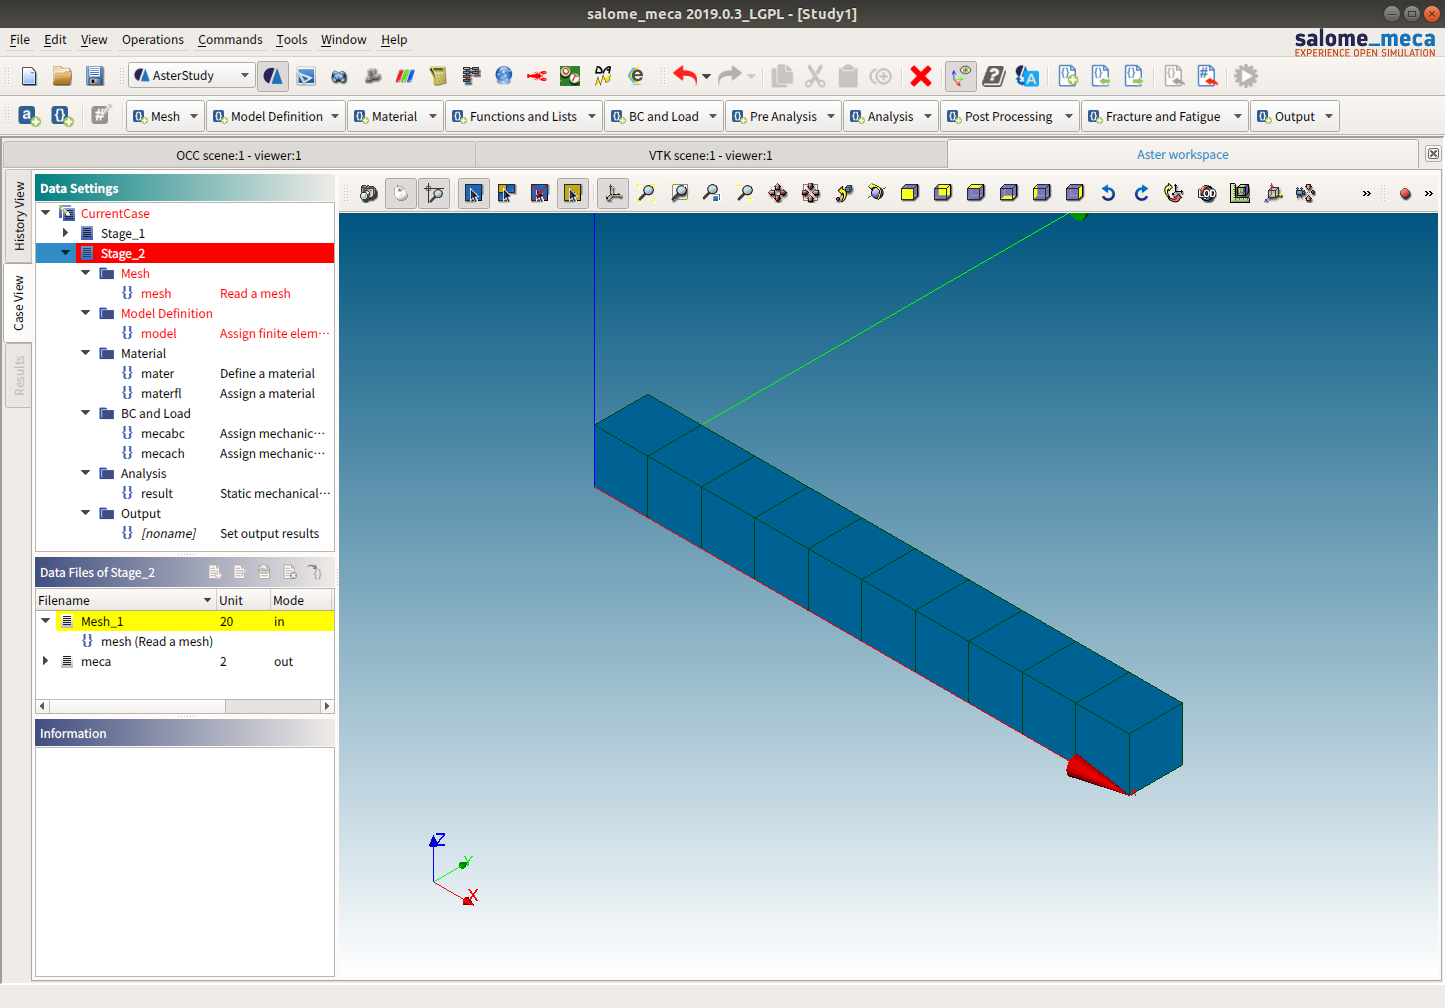
\includegraphics[width=0.7\columnwidth]{fig/conflict.png}
\end{figure}
\clearpage
\begin{itemize}
	\item 以下のLIRE\_MAILLAGE(メッシュの読み込み)を削除
	      \begin{lstlisting}[caption =メッシュの読み込み,label=LIRE_MAILLAGE]
    mesh = LIRE_MAILLAGE(FORMAT='MED',
                         UNITE=20)
    \end{lstlisting}
	\item AFFE\_MODELE(有限要素の選択)のコンセプト名をmodelからmodelSに変更
	\item Meshは熱解析で設定したコンセプト名を選択(ここでは、mesh)
	      \begin{lstlisting}[caption =有限要素の選択,label=AFFE_MODELE]
modelS = AFFE_MODELE(AFFE=_F(MODELISATION=('3D', ),
                             PHENOMENE='MECANIQUE',
                             TOUT='OUI'),
                     MAILLAGE=mesh)
    \end{lstlisting}
	\item DEFI\_MATERIAU(材料の定義)のコンセプト名をmaterからmaterSに変更し、線膨張係数を追加
	      \begin{lstlisting}[caption =材料の定義,label=DEFI_MATERIAU]
materS = DEFI_MATERIAU(ELAS=_F(ALPHA=1.73e-05,
                               E=203000.0,
                               NU=0.3))
    \end{lstlisting}
	\item AFFE\_MATERIAU(材料の割り当て)にAFFE\_VERCを追加して、熱解析の結果を継承し、参照温度を20℃に設定。
	      \begin{lstlisting}[caption =材料の割当,label=AFFE_MATERIAU]
materfl = AFFE_MATERIAU(AFFE=_F(MATER=(materS, ),
                                TOUT='OUI'),
                        AFFE_VARC=_F(EVOL=temp,
                                     NOM_VARC='TEMP',
                                     TOUT='OUI',
                                     VALE_REF=20.0),
                        MODELE=modelS)
    \end{lstlisting}
	\item コンセプト名:macabcのAFFE\_CHAR\_MECA(機械的境界条件の割り当て)を修正
	      \begin{lstlisting}[caption =機械的境界条件の割り当て,label=mecabc]
mecabc = AFFE_CHAR_MECA(DDL_IMPO=(_F(DX=0.0,
                                     GROUP_MA=('Fix_X1', )),
                                  _F(DX=0.0,
                                     GROUP_MA=('Fix_X2', )),
                                  _F(DY=0.0,
                                     GROUP_NO=('Fix_Y', )),
                                  _F(DZ=0.0,
                                     GROUP_NO=('Fix_Z', ))),
                        MODELE=modelS)
    \end{lstlisting}
	\item コンセプト名:mecachのAFFE\_CHAR\_MECAを削除
	      \begin{lstlisting}[caption =荷重条件(圧力条件),label=mecach]
mecach = AFFE_CHAR_MECA(MODELE=model,
                        PRES_REP=_F(GROUP_MA=('Fix_X1', ),
                                    PRES=0.0))
    \end{lstlisting}
	\item MECA\_STATIQUE(静的線形構造解析)を修正
	      \begin{lstlisting}[caption =静的線形構造解析,label=MECA_STATIQUE]
result = MECA_STATIQUE(CHAM_MATER=materfl,
                       EXCIT=_F(CHARGE=mecabc),
                       MODELE=modelS)
    \end{lstlisting}
	\item CALC\_CHAMP(場の量の計算)を追加
	      \begin{lstlisting}[caption =場の量の計算,label=CALC_CHAMP]
result = CALC_CHAMP(reuse=result,
                    CONTRAINTE=('SIGM_ELNO', 'SIGM_NOEU'),
                    CRITERES=('SIEQ_ELNO', 'SIEQ_NOEU'),
                    RESULTAT=result)
    \end{lstlisting}
	\item IMPR\_RESU(結果の出力)を修正
	      \begin{lstlisting}[caption =結果の出力,label=IMPR_RESU]
IMPR_RESU(FORMAT='MED',
          RESU=_F(NOM_CHAM=('DEPL', 'SIEQ_NOEU', 'SIGM_NOEU'),
                  RESULTAT=result),
          UNITE=2)
    \end{lstlisting}
\end{itemize}
\clearpage
\subsection{AsterStudyで求解・データ管理}
\begin{itemize}
	\item 計算のインタラクティブなフォローアップ
	\item 実行ケース間の関係のグラフィカル表示
\end{itemize}
\vspace{-\baselineskip}
\begin{figure}[H]
	% 	\caption{}
	% 	\label{}
	\centering
	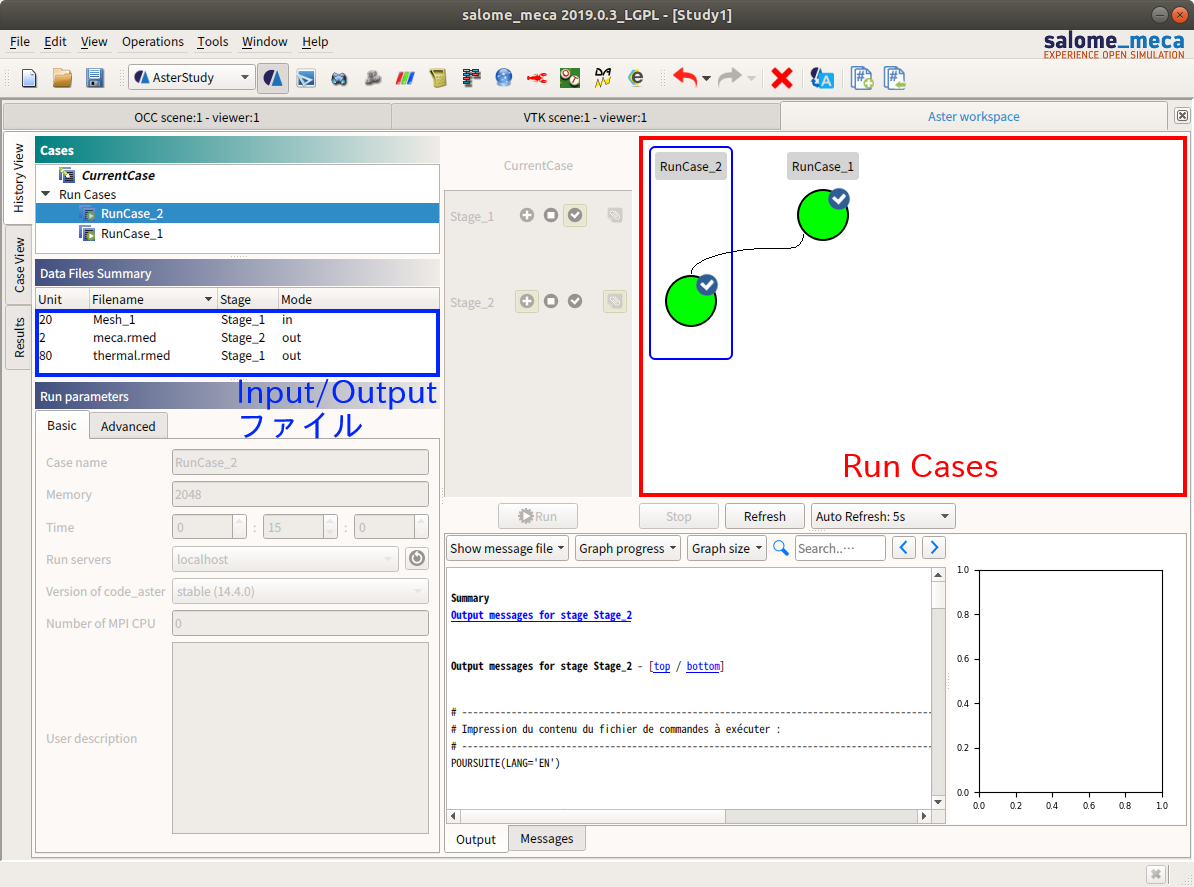
\includegraphics[width=0.75\columnwidth]{fig/runcase.png}
\end{figure}
\clearpage
\subsection{Paravisで結果分析(可視化)}
\begin{itemize}
	\item 熱応力
	      \begin{itemize}
		      \item 理論値:$\sigma=E\alpha\Delta T=20,300\times1.73\times 10^{-5}\times(100-20)=280.952$ (MPa)
		      \item 解析結果:$280.952$ (MPa)
	      \end{itemize}
\end{itemize}
\vspace{-\baselineskip}
\begin{figure}[H]
	% 	\caption{}
	% 	\label{}
	\centering
	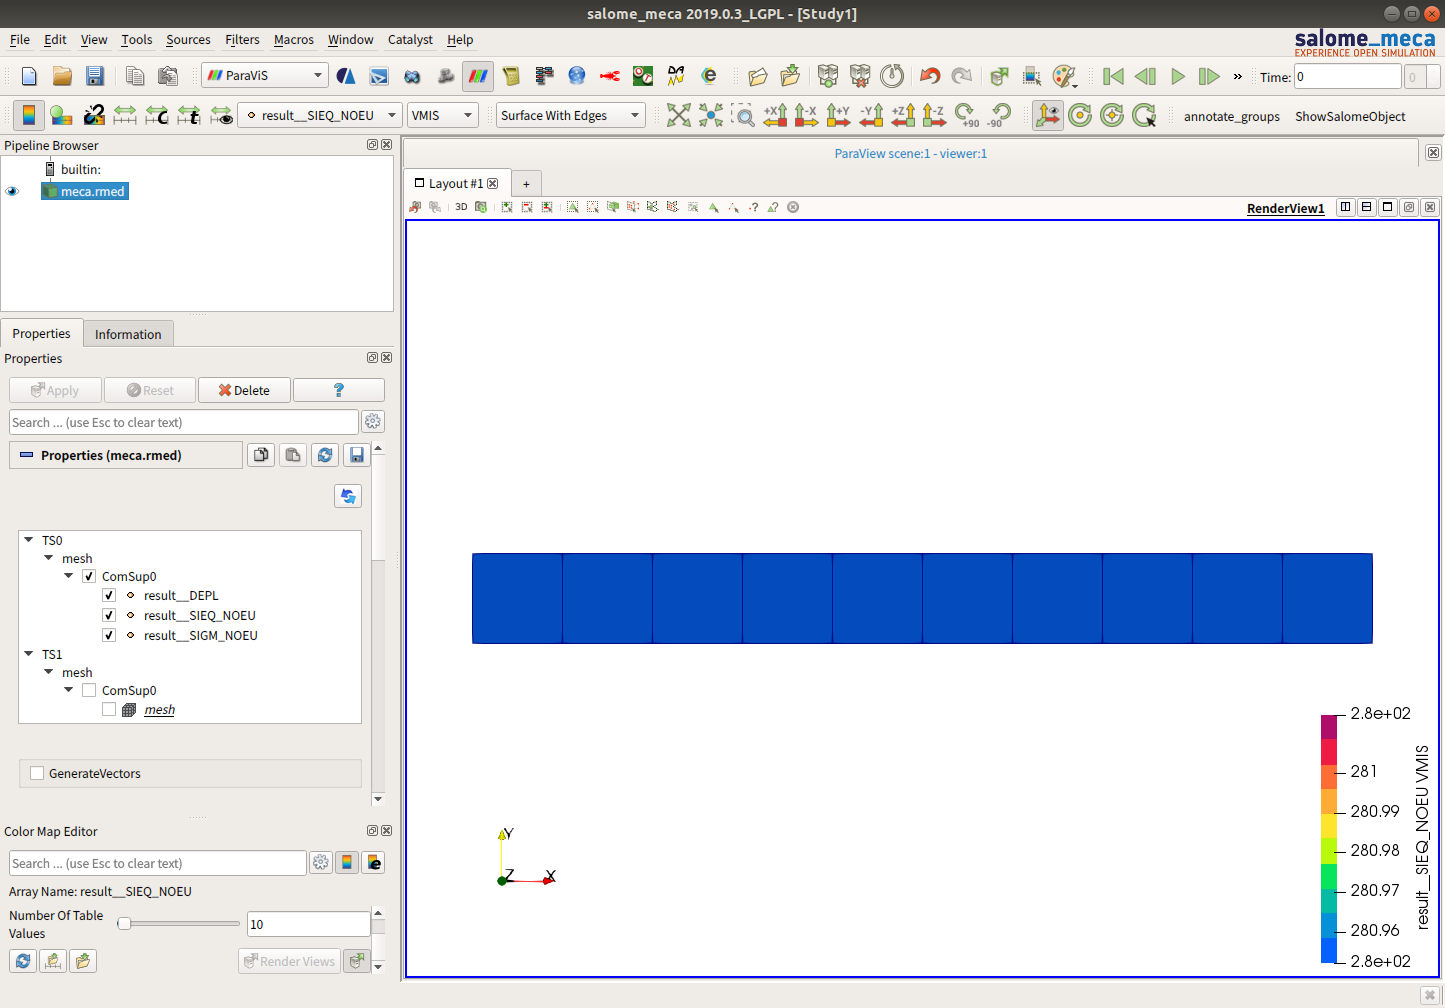
\includegraphics[width=0.75\columnwidth]{fig/vmis.png}
\end{figure}
\section{追加計算}
\subsection{自由端}
\begin{itemize}
	\item 右端の変位拘束(Fix\_X2にDX=0)を削除して計算
	\item X方向変位(100倍表示)
	      \begin{itemize}
		      \item 理論値:$\Delta X=\alpha \Delta T L=1.73\times 10^{-5}\times(100-20)\times 100=0.1384$ (mm)
		      \item 解析結果:$0.1384$ (mm)
	      \end{itemize}
\end{itemize}
\vspace{-\baselineskip}
\begin{figure}[H]
	% 	\caption{}
	% 	\label{}
	\centering
	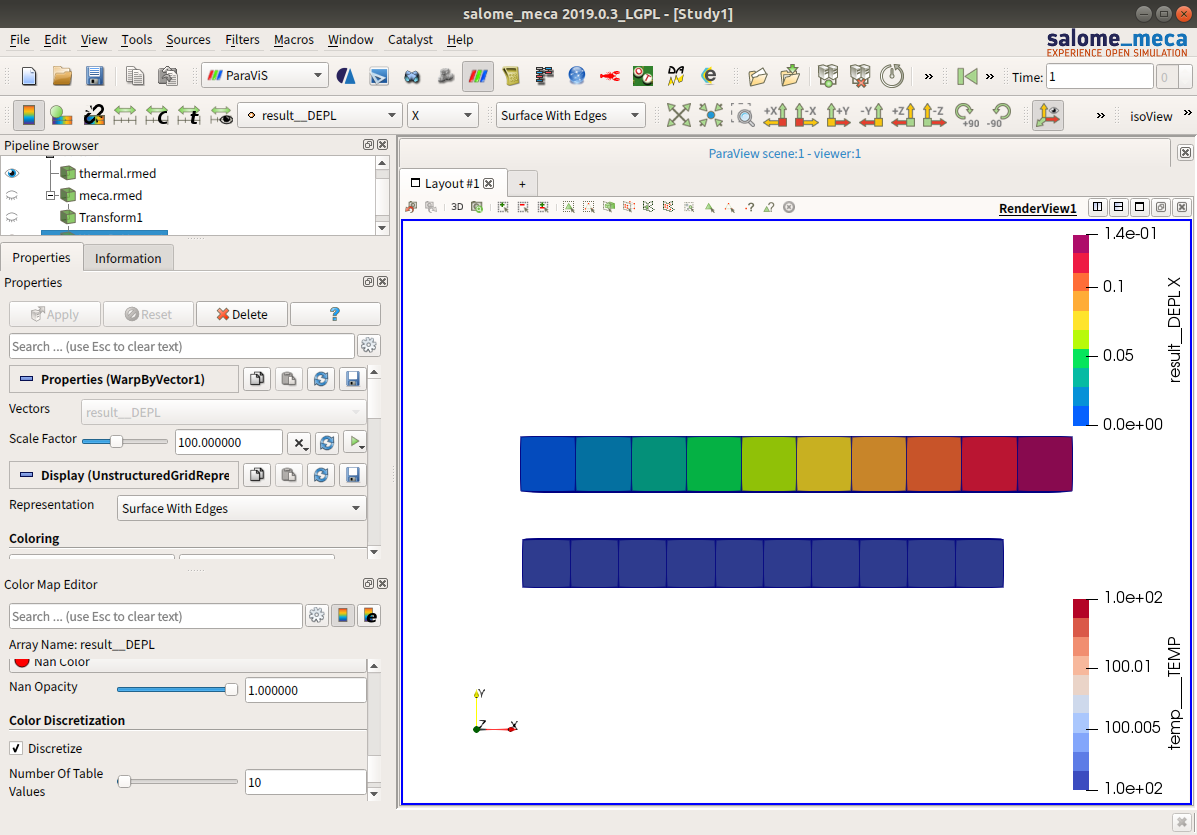
\includegraphics[width=0.65\columnwidth]{fig/Free.png}
\end{figure}